
\chapter{Related Work}
\label{ch:related}

One of the most important papers out there for getting to know the field of fairness in machine learning is the survey paper by \citet{Mehrabi:2021:CSUR}. This paper serves as a gateway to a lot of the current research in the field, a lot of which will be summarised in this section of the thesis.

\section{Bias in Data}

Some of the sources of bias have been discussed already in section \ref{ch:intro} but here we will go through more of them and in more detail. We have the following biases according to \citet{Mehrabi:2021:CSUR}:

\subsection{Historical Bias}

Historical Bias is the already existing bias and socio-technical issues in the real word. These issues affect the data-generation process. So even given a perfect sampling method, the bias in the dataset will still exist. \cite{Suresh:2019:arXiv}

\subsection{Representation Bias}

This is a bias that occurs due to the way the sample has been acquired. \cite{Suresh:2019:arXiv} Data collection is a non-trivial task and sampling a diverse dataset across large geographical regions and taking into account diversity in terms of race, culture, gender etc will in many cases not be possible. Still, the dataset will suffer from not representing the true distributions in the population.

\subsection{Measurement Bias}

This source of bias originates in the way the particular features have been measured and utilised. \cite{Suresh:2019:arXiv} An example of this would be to use salary as a feature to assess risk of defaulting on a loan. This feature will be biased towards women since women has historically experienced having lower salaries than men.

\subsection{Population Bias}

Population bias arises when the sampled population have different properties than the original target population. \cite{Olteanu:2019:FDATA} An example of this would be to sample data from different social media platforms, which have different user demographics. I.e men using reddit and women using instagram.

And there are many other sources of bias and some of these are very hard to avoid. It is reasonable to assume that most available datasets today are biased, which makes the approach described in section \ref{sec:probmac} important.

\section{Algorithmic Fairness}

Discrimination has many different definitions, and while no gold-standard defintion exist, it is often defined as an absence of any prejudice or favouritism towards individuals or groups based on some intrinsic traits. \cite{Mehrabi:2021:CSUR, Nripsuta:2019:AIES} This definitions is core in the many different mathematical definitions of fairness. Some of these are summarised below

\textbf{Equalized Odds}: According to \citet{Mehrabi:2021:CSUR, Hardt:2016:NIPS} A predictor $\hat{Y}$ satisfies equalised odds with respect to a sensitive attribute $A$ and outcome $Y$ if $\hat{Y}$ and $A$ are conditionally independent on $Y$. i.e

\begin{equation}
    P(\hat{Y}|A=0, Y=y) = P(\hat{Y}|A=1, Y=y), y \in {0, 1}
\end{equation}

\textbf{Equal Opportunity}: According to \citet{Mehrabi:2021:CSUR, Hardt:2016:NIPS} A binary predictor $\hat{Y}$ satisfies equal opportunity with respect to $A$ and $Y$ if

\begin{equation}
    P(\hat{Y}=1|A=0, Y=1) = P(\hat{Y}=1|A=1, Y=1)
\end{equation}

\textbf{Demographic Parity}: According to \citet{Mehrabi:2021:CSUR, Dwork:2012:ITCS} A predictor $\hat{Y}$ satisfies demographic parity if 

\begin{equation}
    P(\hat{Y}|A=0) = P(\hat{Y}|A=1)
\end{equation}

And many more metrics exist. A challenge is that according to \citet{Mehrabi:2021:CSUR, Kleinberg:2017:LIPIcs} it is impossible to satisfy some of these fairness constraints. One should therefore be considerate when using a certain metric. Synthesising these definitions to one gold-standard remains an open research question. For this thesis. Demographic parity is especially important as it is fundemental in the model described in section \ref{sec:probmac}.

\section{Methods for Fair Machine Learning}

Machine Learning is a large domain encompassing many sub-domains. These include \textit{Classification, Regression, PCA, Clustering, Deep Learning} and many more. In this thesis, the focus will be on fair classification. This is kind of an arbitrary choice but it has been chosen since a lot of real-world decision making processes are classification problems. 

\textit{Fair Classification:} Some of the most important work in the field of fair classification summarised by \cite{Mehrabi:2021:CSUR}. Some important previous work for this thesis is the Naive Bayes approach for fair classification by \citet{Calders:20210:DMKD} In this work the authors investigated how to modify the naive bayes classifier in order to perform classification that is restricted to be independent from the sensitive attributes. In this paper they measure discrimination by \textit{discrimination score} which is defined as

\begin{equation}
    P(C=+|S_+) - P(C=+|S_-)
\end{equation}

Which assumes that a classifier is fair if the outcome is independent of the sensitive attribute. i.e \textit{Demographic Parity} as described above. The main limitation of this paper is that the classifier on the non-sensitive attributes is a naive-bayes classifier. Which means it assumes that all the features are independent. This makes it one of the simplest bayesian networks out there as well as scalable since the number of parameters is scaled linearly with the number of features. This limitation is adressed further in section \ref{sec:probmac}.

Other important works are the works of \cite{Zafar:2017:NIPS} and \citet{Dwork:2018:PMLR}. \citet{Zafar:2017:NIPS} introduced new notions on how to define fairness, arguing that the traditional parity based notion is  quite stringent, limiting the overall decision making accuracy. They tie in elements from envy-freeness literature in economics and game theory and propose preference-based notions of fairness. 

\citet{Dwork:2018:PMLR} provide a simple and efficient decoupling technique, which can be added on top of any black-box machine learning algorithm, to learn different classifers for different groups. Transfer learning is used to mitigate the problem of having too little data on any one group.

Important to this thesis is the work of \citet{Choi:2021:AIII} Which is a follow up paper to \cite{Calders:20210:DMKD}. They have generalised the limitation of the first paper where a naive-bayes classifier was necessary. Their framework can be generalised to any local probabilistic network. This will be discussed in more detail in section \ref{sec:probmac}

\section{Probabilistic Machine Learning}
\label{sec:probmac}

In this thesis, we will focus on probabilistic machine learning, therefore a brief introduction to this field is in place. According to \citet{Murphy:2012:Book} machine learning is usually divided into two main types. \textbf{Predictive} or \textbf{Supervised learning} approach \cite[p.~2]{Murphy:2012:Book}, the goal is to learn a mapping from inputs $x$ to outputs $y$ given a labeled set of input-output pairs

\begin{equation}
    \mathcal{D} = {(x_i, y_i)}_{i=1}^N
\end{equation}

The second type is the \textbf{descriptive} or \textbf{unsupervised learning} where we are only given the data itself without labels

\begin{equation}
    \mathcal{D} = {x_i}_{i=1}^N
\end{equation}

here the goal is to find interesting patterns in the data that is inherent to the data itself without the need of labels. This problem is not as well defined as the predictive case and there is no obvious error metric. The third type is \textbf{reinforcement learning} where you let an agent explore a space and desired behaviour is rewarded through a performance or reward metric. 

A common way to perform supervised learning is to treat  $y$ as a random variable and estimate a mapping 

\begin{equation}
    f: x \rightarrow y
\end{equation}

One example of this is Linear Regression. Which maps input vectors $x$ to outputs $y$ using the following mapping \cite[p.~19]{Murphy:2012:Book}

\begin{equation}
    f: y = \mathbf{w}^Tx + \epsilon = \sum_{j=1}^N w_j x_j + \epsilon
\end{equation}

and often $\epsilon$ is assumed to be gaussian and the model can be rewritten as 

\begin{equation}
    p(y|x, \theta) = \mathcal{N}(y|\mu(x), \sigma^2(x))
\end{equation}

One common way to estimate the parameters of a statistical model is to calculate the maximum likelihood estimate of the model parameters \cite[p.~217]{Murphy:2012:Book}

\begin{equation}
    \hat{\mathbf{\theta}} = \argmax_{\theta} \log p(\mathcal{D}|\theta)
\end{equation}

and for linear regression, minimising the sum of squared errors has an explicit solution \cite[p.~220]{Murphy:2012:Book}

\begin{equation}
    \hat{\bf{w}}_{\text{OLS}} = (\bf{X}^T\bf{X})^{-1}\bf{X}^T\bf{y}
\end{equation}

This estimate gives us a point estimate of the model parameters. I.e one dataset produces one point estimate. This is traditionally what many machine learning algorithms do, take a dataset and calculate the most likely point estimate of the model parameters. It is reasonable to assume that the model parameters that is returned from one dataset is different to the true model parameters and it would in many cases be beneficial to know how uncertain the model parameters are. This is where the \textbf{probabilistic} approach comes in.

In a probabilistic approach, we treat the input data and labels as random variables, but also the model parameters. After training, we will have a distribution of model parameters which we can sample from and simulate different realisations of our models. One example of this is \textbf{Bayesian Linear Regression}

In bayesian linear regression, the likelihood of $y$ is given by \cite[p.~232]{Murphy:2012:Book}

\begin{equation}
    p(\bf{y}|\bf{X}, \bf{w}, \mu, \sigma^2) = \mathcal{N}(\bf{y}|\mu + \bf{X}\bf{w}, \sigma^2 \bf{I}_N)
\end{equation}

and using a gaussian prior distribution since it is a conjugate prior, the posterior becomes \cite[p.~232]{Murphy:2012:Book}

\begin{equation}
    p(\bf{w}|\bf{X}, \bf{y}, \sigma^2) \propto \mathcal{N}(\bf{w}|\bf{w_0}, \bf{V_0}) \mathcal{N}(\bf{y}|\bf{Xw}, \sigma^2\bf{I})
\end{equation}

And we have a full distribution of model parameters, which gives us insight into the uncertainty of the model. This property is desired for assessing fairness and uncertainty later in this thesis.

\section{Graphical Models}

A graphical model is a way to represent a joint probability distribution. Nodes represent random variables and the edges between the random variables is for dependencies and the lack of edges means the random variables are conditionally independent. \cite[p.~308]{Murphy:2012:Book} There are many different graphical models and all of them tie probability theory and graph theory together in a comprehensive manner. In this section some different models are described

\section{Bayesian Networks}

\begin{figure}[h!]
    \centering
    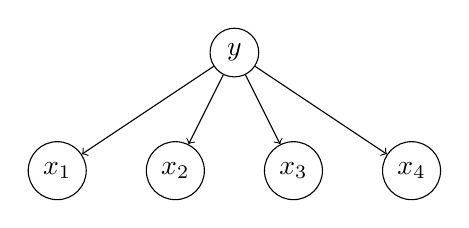
\begin{tikzpicture}[nodes={draw, circle}, ->]
        \node {$y$}
            child {node {$x_1$}}
            child {node {$x_2$}}
            child {node {$x_3$}}
            child {node {$x_4$}};
    \end{tikzpicture}
    \caption{Bayesian network with $4$ features representing the naive-bayes classifier}
    \label{fig:my_label}
\end{figure}

Graphical models gives us a graphical way to represent the joint pdf. It models the conditional dependencies between random variables. From this graph, we see that the joint probability distribution of this classifier is

\begin{equation}
    p(y, x_1, x_2, x_3, x_4) = p(y)p(x_1|y)p(x_2|y)p(x_3|y)p(x_4|y)
\end{equation}

\subsection{Markov Random Fields}

add more later

\subsection{Factor Graphs}

add more later

\subsection{Sum-Product Networks}

add more later

\section{Modeling Discrimination Process}

Now that probabilistic machine learning and graphical models have been introduced, it is time to introduce the work of \citet{Choi:2021:AIII} in more detail. As discussed previously in this section. There are many sources of bias in data and it is reasonable to assume that almost all datasets out there is biased. \citet{Choi:2021:AIII} describes a way of learning fair probability distributions from biased data by explicitly modeling a latent variable that represents a hidden, unbiased label. In particular, they aim to achieve demographic parity by enforcing
certain independencies in the learned model.

\begin{figure}[h!]
    \centering
    \begin{tikzpicture}[nodes={draw, circle}, ->]
        \node (S) {$S$};
        \node (Df) [right=of S] {$D_f$};
        \node (X)  [below=of S] {$X$};
        \node (D)  [below=of Df] {$D$};
        
        \draw (S) -> (X);
        \draw (S) -> (D);
        \draw (Df) -> (X);
        \draw (Df) -> (D);
    \end{tikzpicture}
    \caption{Bayesian network structures that represent the proposed
fair latent variable approach from \cite{Choi:2021:AIII}}
    \label{fig:choinetwork}
\end{figure}

In other words, they model the process on how biased datasets are generated. The biased labels present in the dataset are dependent on the sensitive attributes $S$ and the true fair labels $D_f$. The latent variable $D_f$ is used for decision making on future instances by inferring $P(D_f|e)$ given some evidence.

The paper states that any probabilistic model can be used but that this model needs to satisfy the independence assumptions in the bayesian network.